\documentclass[preprint,prd,showpacs]{revtex4-1}
\usepackage{graphicx}
\usepackage{listings}

\newcommand{\pt}{\ensuremath{p_T}}
\newcommand{\met}{\ensuremath{E_{T}^{miss}}}
\newcommand{\gev}{~\mathrm{GeV}}
\newcommand{\tev}{~\mathrm{TeV}}
\newcommand{\ifb}{~\mathrm{fb}^{-1}}
\newcommand{\mhz}{~\mathrm{MHz}}
\newcommand{\khz}{~\mathrm{KHz}}
\newcommand{\kt}{k_{T}}
\newcommand{\et}{E_{T}}

\newcommand{\trimmedgraphic}[2][]{
  \includegraphics[width=0.4\textwidth,trim={0.5cm 1cm 1.5cm 1cm},clip,#1]{#2}
}


\begin{document}
\title{Commercial associative memory performance for applications in track-based triggers at the Large Hadron Collider}
\author{Jordan Webster}
\affiliation{Argonne National Laboratory}
\author{Jinlong Zhang}
\affiliation{Argonne National Laboratory}

\date{\today}
\begin{abstract}
  Dense track environments in $pp$ collisions at the Large Hadron Collider (LHC) motivate the use of triggers with dedicated hardware for fast track reconstruction. The ATLAS Collaboration is in the process of implementing a Fast Tracker (FTK) trigger upgrade, in which Content Addressable Memories (CAMs) will be used to rapidly match hit patterns with large banks of simulated tracks. The FTK CAMs are produced primarily at the University of Pisa. However, commercial CAM technology is developing at a fast pace for computer networking applications. This document contains proceedings for a poster presented on new studies comparing FTK CAMs to cutting edge ternary CAMs developed by Cavium. The comparison is intended to guide the design of future track-based trigger systems for the next Phase at the LHC.
\end{abstract}

\maketitle

\section{Introduction}\label{sec:Introduction}

The Large Hadron Collider (LHC) is designed to collide protons 40 million times per second, which produces an enormous amount of data. Due to hardware limitations the ATLAS and CMS experiements are only capable writing approximately 100 collisions (or events) to disk per second. As a result, both experiments are forced to implement multi-level trigger systems designed to rapidly identify events with interesting physics. Events that are not flagged by these triggers are discarded on the fly so that the event rate is reduced before data is saved to disk.

Reconstructing charged particle tracks in silicon detector layers is critical for making trigger decisions because tracks tend to be associated with interesting objects, like electrons, muons, and $b$-jets. Tracks can also be used to estimate missing transverse energy and to identify primary vertices. Unfortunately, track reconstruction is computationally expensive. Figure~\ref{fig:pattern_cartoon} shows a simple cartoon of the problem at hand. Hits in each silicon layer are represented by red stars. One of the primary challenges in track reconstruction is to determine which combinations of hits come from plausible track candidates. Typical collisions contain thousands of silicon detector hits and hundeds of tracks with transverse momentum above $1\gev$. Performing a full helical fit of every single combination of hits in the silicon detector layers is impossible even at a $100\khz$ event rate (nominal output rate of the ATLAS Level-1 Trigger).

\begin{figure*}[!htb]
\begin{center}
\includegraphics[width=0.5\textwidth]{figures/pattern_cartoon}
\caption{Two-dimensional cartoon of an example track candidate in a 5-layer silicon detector. The red stars represent pixel hits. Each layer is evenly segmented into boxes that represent coarse groups of nearby pixels. These groups are meant to represent FTK-style \textit{super-strips}.}
\label{fig:pattern_cartoon}
\end{center}
\end{figure*}

The solution is to build dedicated hardware like the Fast Track Trigger (FTK) system for ATLAS~\cite{Shochet:1552953}, which can do \textit{approximate} track reconstruction at $100\khz$. A key component of all hardware-based track triggers, including FTK, is Associative Memory (AM), or Content Addressable Memory (CAM). CAMs are a special type of computer memory used for high speed search applications. They are built for comparing input data against a table of stored data to look for matching patterns. The CAMs in FTK are loaded with large banks of precomputed hit patterns associated with simulated tracks. When hits from the silicon detector readout system are passed into FTK, the CAMs return a list of matched hit patterns. Each matched pattern (or \textit{road}) therefore represents a track candidate, and the hit values can be used to compute helix parameters and a $\chi^{2}$ goodness-of-fit. In practice, the these parameter values are only estimated with a linear approximation to save time.

Figure~\ref{fig:am_cartoon} shows a drastically simplified cartoon model of a CAM. The memory is composed of a strucured lattice of comparators. Hits arriving from the left are compared with precomputed hit patterns, represented by vertical strings of characters. A pattern fires if there is a matching hit in each detector layer. Additional logic can be used to allow patterns to fire when they are missing hits in one or more layers due to detector innefficiency.

\begin{figure*}[!htb]
\begin{center}
\includegraphics[width=0.5\textwidth,trim={7cm 6cm 7cm 6cm},clip]{figures/am_cartoon}
\caption{Simplified cartoon of a CAM used for a identifying track candidates using 5 silicon detector layers. The cartoon shows 8 pre-stored hit patterns. Each pattern has one character (representing one hit coordinate) per layer. Hits enter the CAM on the left side of the cartoon. Matches are triggered if a pattern has a matching hit in each layer.}
\label{fig:am_cartoon}
\end{center}
\end{figure*}

FTK uses dedicated CAM chips built specifically for use in the ATLAS trigger system. However, commercial CAMs developed primarily for computer networking applications could be a viable alternative in future detector upgrades. The remainder of this note contains performance studies of a cutting-edge commercial tCAM chip developed by Cavium. Section~\ref{sec:TestSetup} describes the software and hardware setup used to run performance tests. Section~\ref{sec:Results} contains results, and a short discussion of the results is in Section~\ref{sec:Discussion}.

\section{Test Setup}\label{sec:TestSetup}

A test stand at Argonne National Laboratory was developed to measure the performance of a particular ternary-CAM (tCAM) developed by Cavium. Ternary CAMs allow for pattern matching with ``don't care'' (DC) bits, which are currently used in FTK to reduce the number of patterns stored in memory. Tests are done using 128~bit FTK-like patterns, with a varied number of DC bits per pattern. The patterns themselves are generated from FTK simulation using an 8-layer pattern matching scheme and the proposed detector geometry for Phase-II (Step 1.5). The DC bits, when turned on, are arbitrarily added to the end of each pattern.

\subsection{Hardware}

The hardware setup primarily consists of a host computer (atlas30.hep.anl.gov), a Network Processor board (OCTEON CN6800), and a Neuron Search Processor board (CNSP1600). Figure~\ref{fig:board_pic} shows a labeled photograph of the latter two components. The host computer is used to control the the Network Processor via a null modem connection. Minicom is used to run the serial console. The Network Processor is connected to the CNSP1600 via QSFP connectors. The tCAM is a component of the CNSP1600 board.

\begin{figure*}[!htb]
\begin{center}
\includegraphics[width=0.8\textwidth]{figures/TCAM_pic}
\caption{Photograph of the Network Processor board (OCTEON CN6800) and the attached Nueron Search Processor board (CNSP1600).}
\label{fig:board_pic}
\end{center}
\end{figure*}

The Network Processor contains 22 cores and on-board flash memory. It is capable or running a linux kernel and/or running applications to test lookups on the CNSP1600. The tCAM chip is divided into 4 memory clusters of equal size.

\subsection{Software}

A patched version of the OCTEON SDK v2.3.0 software library is used to build a linux kernel for the Network Processor and to compile code for testing the CNSP1600 lookup rate. A rough installation guide is outlined below. The packages and patches listed can only be obtained from Cavium.
\begin{enumerate}
\item Install OCTEON\_SDK v.2.3.0
\item Unpack and install dependent packages:
  \begin{itemize}
  \item OCTEON-SDK-2.3.0-427
  \item OCTEON-LINUX-2.3.0-427
  \item OCTEON-COMPONENTS-COMMON-2.3.0-62
  \item OCTEON-PCI-BASE-2.3.0-84
  \end{itemize}
\item Apply release5 patches:
  \begin{lstlisting}
cd ${OCTEON_ROOT}
patch -p0 < \
  /path/to/NSP-SDK-2.2.1/patches/octeon/executive-2.3.0-p5.patch
patch -p0 < \
  /path/to/NSP-SDK-2.2.1/patches/octeon/linux-2.3.0-p5.patch
  \end{lstlisting}
\item Apply a bug fix to allow lookup rate tests with arbitrary pattern banks (the patch file here must be acquired from Cavium):
  \begin{lstlisting}
cd /path/to/NSP-SDK-2.2.1
patch -p0 < fix_bug18568.patch
  \end{lstlisting}
\end{enumerate}

For this study an OCTEON Linux kernel was compiled and loaded onto the Network Processor (see Cavium documentation for details), and the kernel was used to run test applications. However, it is also possible to run test applications directly from the bootloader, thus avoiding the need to build OCTEON Linux. Some rough instructions are provided below for compiling and running the ``nsp\_perf\_test'' application included in the NSP-SDK-2.2.1 package. This application is nominally used to test the CNSP1600 lookup rate using a rule table that consists of IP addresses. However, the rough instructions below can be used to compile and test with an arbitrary rule file. Note that ``rule'' is the Cavium term for pattern. A rule file is the analog of an FTK pattern bank.
\begin{enumerate}
\item Generate a test packet header file that represents your rule file:
  \begin{lstlisting}
/path/to/NSP-SDK-2.2.1/nsp-utils/nspc -i [input rules file] \
  -o output_rules.bin
/path/to/NSP-SDK-2.2.1/nsp-utils/nspt -c `` \
  lib -add db -file output_rules.bin -name db0; \
  lib -add group -name g0 db0; \
  dev -lookup [input traces file] -group g0'' \
    -dbg=l > test_pkt_data1.h
  \end{lstlisting}
\item Modify header so it is formatted correctly:
  \begin{itemize}
  \item Ensure the length of ``pkt\_data'' is correct
  \item Remove any partially constructed trailing element from ``pkt\_data''
  \end{itemize}
\item Compile nsp\_perf\_test with this new header:
  \begin{lstlisting}
cp test_pkt_data1.h \
  /path/to/NSP-SDK-2.2.1/nsp-agent/platform/app/pkt_data_hdrs/
cd /path/to/NSP-SDK-2.2.1/nsp-agent/platform/app/nsp_perf_test/
make clean && make
  \end{lstlisting}
\item Load the compiled application onto the Network Processor (e.g. using USB to transfer the executable).
\item Boot the application (e.g. from minicom). You can specify the number of cores to use. One core should be reserved to gather statistics. Out of the remaining cores, half will be used to send packets and half will be used to recieve packets.
  \begin{lstlisting}
# Run on 21 cores (with 10 cores sending packets)
bootoct 0 coremask=0x1fffff endbootargs --recv_mask 0x3ff
# Run on 17 cores (with 8 cores sending packets)
bootoct 0 coremask=0x1ffff endbootargs --recv_mask 0xff
  \end{lstlisting}
\end{enumerate}

An example rule file can be found in Appendix~\ref{app:ExampleRulesFile}. Furthermore, a script for generating rule files from FTK-format pattern banks can be found here: \url{https://github.com/jwebste2/CAMTools/blob/master/GenRulesFromPatterns.py}.

Note that the size and lookup rate of the CNSP1600 can also be estimated using a simulation library built into the software. The lookup rate numbers measured from simulation in this experiment were found to be significantly different from the lookup rates measured on the board with ``nsp\_perf\_test''. Regardless, the steps required to simulate the lookup rate can be found in the script linked above.


\section{Results}\label{sec:Results}

The Cavium CNSP1600 performance was measured for FTK pattern banks with 500, 1K, 50K, 100K, 150K, 200K, and 235K patterns. The number of DC bits was varied from 0 to 16 bits in steps of 4-bit steps. Figure~\ref{fig:nsp_perf_plots} contains two plots showing the resulting measurements of cluster usage and lookup rate. The 4 memory clusters on the CNSP1600 have a combined storage capacity of roughly 237K patterns (3.79~MB), assuming the patterns have no DC bits. The storage capacity increases when more DC bits are used because less data needs to be loaded into memory. Due to the way the memory is structured the correlation is not perfectly linear. When using 16 DC bits per pattern the memory can hold roughly 281K patterns. The lookup rate on the other hand has little variation with respect to both pattern bank size and number of DC bits. The rate is found to be between 22 and 27 million lookups per second for all tested banks.

\begin{figure*}[!htb]
\begin{center}
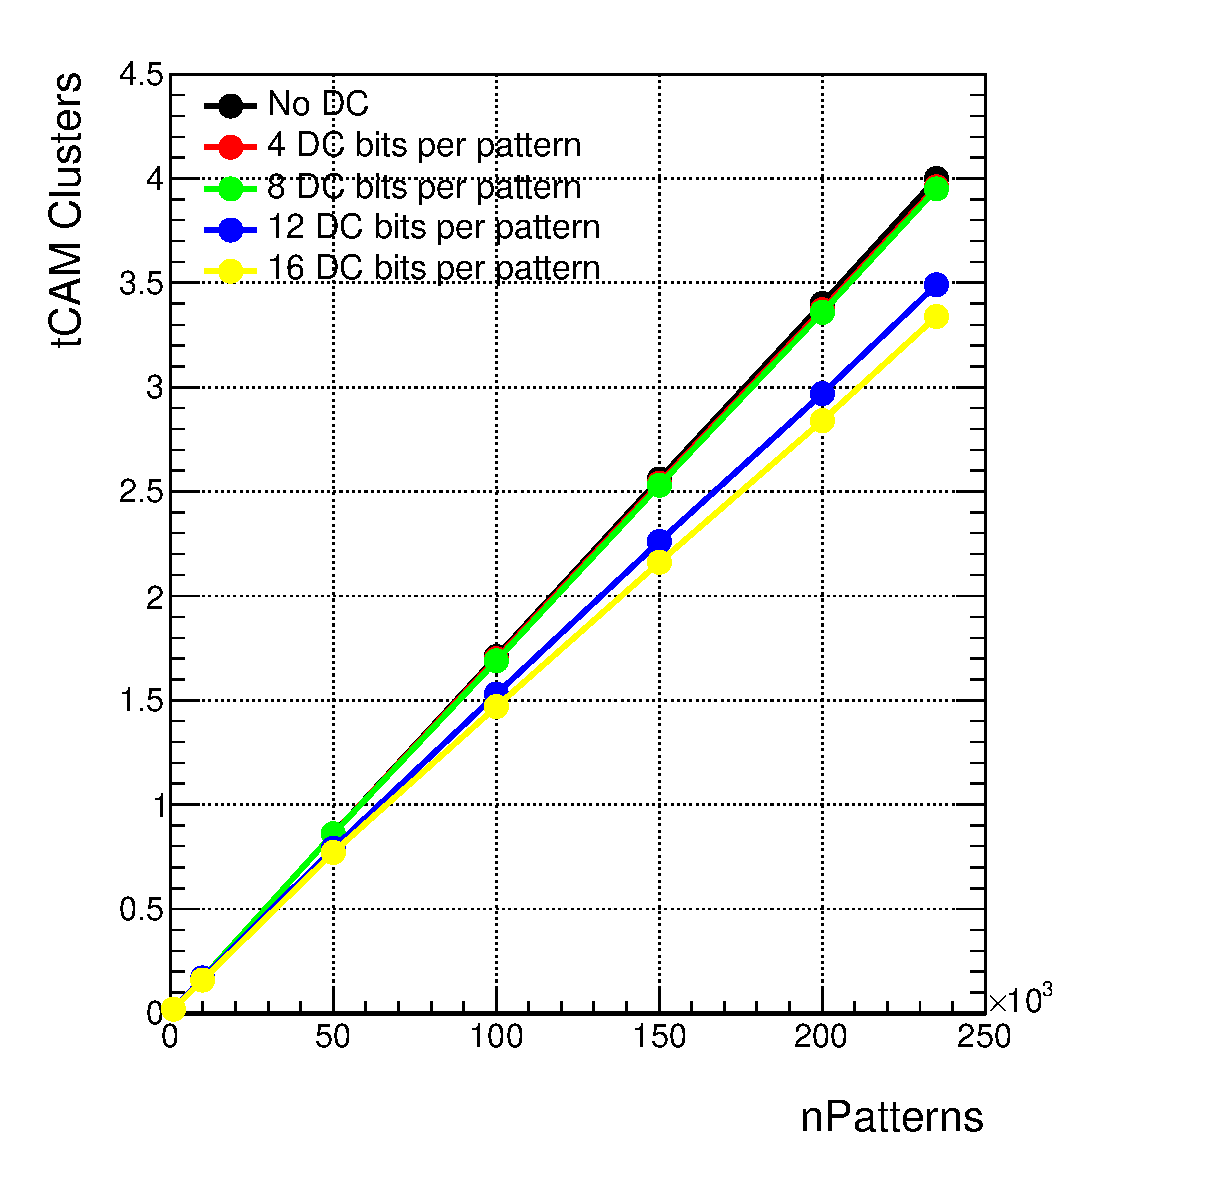
\includegraphics[width=0.45\textwidth]{figures/PlotTcamData_eps/001}
%\hspace{1cm}
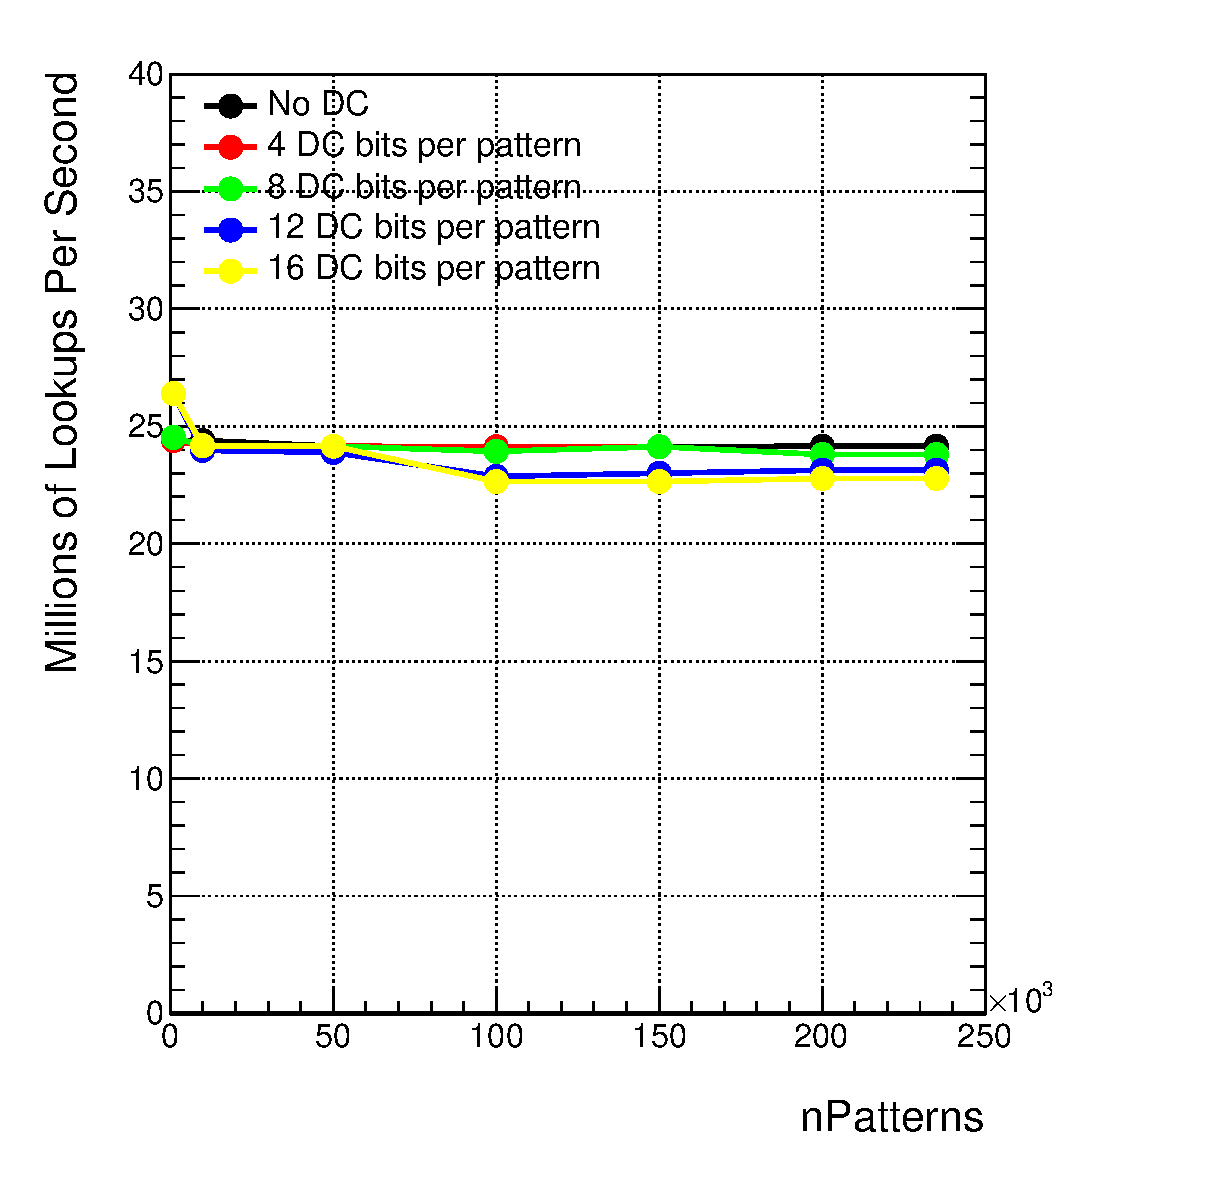
\includegraphics[width=0.45\textwidth]{figures/PlotTcamData_eps/002}
\caption{CNSP1600 cluster usage (left) and lookup rate (right) as a function of the number of patterns loaded onto the chip, and the number of DC bits used for each pattern.}
\label{fig:nsp_perf_plots}
\end{center}
\end{figure*}


\section{Discussion}\label{sec:Discussion}

For an FTK-like track triggering application, the Cavium CNSP1600 is found to be able to store roughly 237K hit patterns and perform lookups at a rate of roughly $24\mhz$. For comparison, the latest CAMs developed for FTK (AM07) can store 128K patterns and have a lookup rate of $100\mhz$~\cite{FIXME}. In summary, Cavium's memory has over 85\% more storage per chip but performs lookups at a quarter of the FTK rate. This means the Cavium chips would be able to operate at an event rate of $\sim25\khz$ assuming no additional parallelization. This is not fast enough to keep up with the $100\khz$ ATLAS Level-1 trigger rate, but increasing the number of CAMs used in the trigger system (for greater parallel processing) could help. 

FIXME: Cost comparison? (FTK chips are $\sim$\$1000 per chip minus person-power)

%Meanwhile the estimated cost
%Results indicate that commercial tCAMs from Cavium have sufficient storage capacity, but are only fast enough to perform FTK-like track reconstruction at a ~25 KHz event rate. Furthermore, Cavium's chips are  roughly 20× more expensive than the latest FTK AM chips (excluding R\&D costs). However, since the cost of commercial technology drops faster than the cost of dedicated hardware, the commercial options are likely to become more promising in the near future.

\section{Acknowledgments}
This work was supported by the U.S. Department of Energy, Office of Science under contract DE-AC02-06CH11357.

\bibliography{proc}

\section{Appendix: Example Rule File}\label{app:ExampleRuleFile}

Rule files are textual lists of patterns that are converted to binary format and then loaded onto the tCAM. The format of these files is described in detail in Cavium's NSPC documenation. The first line of the file specifies the format of all patterns in the bank and the rest of the file contains a list of patterns. Below is an example rule file corresponding to an FTK pattern bank with 10 8-layer patterns (18-bits per layer) and 4 DC bits per pattern.

\begin{lstlisting}[mathescape,basicstyle=\small\ttfamily]
18e 18e 18e 18e 18e 18e 18e 18m
0x105f2 0x1485b 0x19295 0x18ead 0x1f055 0x1ec6d 0x26d56 0x26d56/0x3fff0
0x10dcc 0x15804 0x1b1dd 0x1adf5 0x232c1 0x22ed9 0x2dea2 0x2dea2/0x3fff0
0xb7da 0xee8b 0x130f4 0x130f4 0x19299 0x18eb1 0x21382 0x21382/0x3fff0
0x105fb 0x15034 0x1a625 0x1a23d 0x22321 0x21f39 0x2c732 0x2c732/0x3fff0
0xcf47 0x10dc8 0x14861 0x14479 0x1a61f 0x1a237 0x21b50 0x21b50/0x3fff0
0x111af 0x15fd0 0x1b9a9 0x1b5c1 0x23e77 0x23a8f 0x2ee40 0x2ee40/0x3fff0
0x111b3 0x15804 0x1aa0d 0x1a625 0x21f39 0x21b51 0x2afc2 0x2afc2/0x3fff0
0xb7d6 0xee87 0x130f0 0x130f0 0x19297 0x18eaf 0x21380 0x21380/0x3fff0
0xd330 0x10dc8 0x14479 0x14091 0x19a67 0x1967f 0x1f058 0x1f058/0x3fff0
0xa06b 0xc77c 0xee8d 0xeaa5 0x130f1 0x12d09 0x16b8a 0x16b8a/0x3fff0
\end{lstlisting}

\end{document}




